\documentclass[conference]{IEEEtran}
\IEEEoverridecommandlockouts
% The preceding line is only needed to identify funding in the first footnote. If that is unneeded, please comment it out.
\usepackage{cite}
\usepackage[acronym]{glossaries}
\usepackage{amsmath,amssymb,amsfonts}
\usepackage{algorithmic}
\usepackage{graphicx}
\usepackage{textcomp}
\usepackage{xcolor}
\def\BibTeX{{\rm B\kern-.05em{\sc i\kern-.025em b}\kern-.08em
    T\kern-.1667em\lower.7ex\hbox{E}\kern-.125emX}}
\begin{document}

\title{Weather Data Integration and Assimilation System\\
% \thanks{Identify applicable funding agency here. If none, delete this.}
}

\author{\IEEEauthorblockN{Gihan Karunarathne}
\IEEEauthorblockA{\textit{dept. computer science and Engineering} \\
\textit{university of moratuwa}\\
Moratuwa, Sri Lanka \\
gihan.09@cse.mrt.ac.lk}
\and
\IEEEauthorblockN{Dr. Dilum Bandara}
\IEEEauthorblockA{\textit{dept. computer science and Engineering} \\
\textit{university of moratuwa}\\
Moratuwa, Sri Lanka \\
dilumb@cse.mrt.ac.lk}
}

\maketitle

%%%%%%%%%%%%%%%%%%%%%%%%%%%%%%%%%%%%%%%%%%%%%%%%%%%%%%%%%%%%%%%%%%%%%%%%%%%%%%%%
\begin{abstract}
We describe our experience with implementing an extendable open source Weather Data Integration and Assimilation System, which is known as \acrshort{wdias}. It uses the modern architecture pattern such as microservice in order to achieve the scalability, rather using monolithic architecture or client service architecture. It provides a modular approach to integration data from different sources and export into different formats. Also the inbuilt extension module system allow users to add new features. The open source tools that are using for \acrshort{wdias} allows to run on Cloud Computing platforms without much hassle with the auto scaling feature allow to run \acrshort{wdias} from 1 CPU node to nodes with few hundred CPUs. The paper describes the initial design goals, evolve over few architectures to get desired performance, and explains how the system in way to achieve scalability. Later we analyse the performance test observations with the performance metrics.
\end{abstract}

\begin{IEEEkeywords}
\acrshort{wdias}, weather, microservice, kubernetes, hierarchical database 
\end{IEEEkeywords}

%%%%%%%%%%%%%%%%%%%%%%%%%%%%%%%%%%%%%%%%%%%%%%%%%%%%%%%%%%%%%%%%%%%%%%%%%%%%%%%%
\section{INTRODUCTION}
I'm going to do this today \cite{Haggett1998AnWales}.
Give general idea on weather data integration systems.
Talk about the existing systems. And they're proprietary or close source.
(Don't dedicate another section, otherwise need to do a comparison at the performance analysis)
At the end the structure of rest of the paper

To enhance the accuracy of weather predictions, it is necessary to provide reliable and detailed weather data as inputs to \acrfull{nwm}. These NWMs utilize weather data collected via diverse sources such as automated weather stations, radars, air balloons, and satellite images. Prior to feeding such diverse data (collected from different sources that belong to different stakeholders) into respective NWMs, it is necessary to integrate data into a common format. Moreover, the data integration system’s response time needs to be relatively low to accommodate critical situations like hurricanes, storms, and floods which require rapid and frequent execution of NWMs.

Providing public access to weather data is also useful to enable many third-party applications and research. For example, logistic companies can use that data with their own model to plan and schedule their deliveries. Agricultural insurance companies can warn the farmers in advance, as well as calculate premiums based on anticipated weather patterns.

While Data Integration and Analysis System (DIAS) and Meteorological Assimilation Data Ingest System (MADIS) are some of well-known Weather Data Integration and Assimilation (WDIA) systems, they are proprietary. Further Delft-FEWS is free to use, it is not open source. Hence, users of WDIA are forced to pay heavy licenses and are unable to extend the solutions to cater to their country-specific requirements. Therefore, the objective of this research is to develop a WDIA system for Sri Lanka, as well as make it open source, so that others could use and contribute to the solution.

TODO: Specify the \acrshort{lead} service as a building block approach. \acrshort{fews} more modular approach with general adapter. And \acrshort{wdias} using microservice as module.
Similar to the \acrfull{fews} \cite{WERNER2004DELFT-FEWS:SYSTEM} 

The main purpose of this framework is to provide a platform through which opera- tional forecasting systems can be constructed, and that allows flexibility in the integration of models and data. In contrast to the NWSRFS and the RFFS systems that also follow a modular approach, the Delft-FEWS system contains no inherent hydrological model- ling capabilities within its code base. I

TODO: Update content as below, overview of rest of the paper
This paper first provides a short review of the operational forecasting process and the role of Delft-FEWS within that process. Section 3 provides an overview of the philosophy and the most important components and features of Delft-FEWS, while Section 4 discusses some example applications of the Delft-FEWS system in research and operations. A discussion of the systems strengths and limitations is provided in Section 5. Section 6 finally provides a summary of the paper, as well as an outlook on the future development of Delft-FEWS.
%%%%%%%%%%%%%%%%%%%%%%%%%%%%%%%%%%%%%%%%%%%%%%%%%%%%%%%%%%%%%%%%%%%%%%%%%%%%%%%%
\section{Modules of Weather Data System}
The figure \ref{fi:wdia_components} shows the basic functions of a Weather data integration and assimilation system.
\begin{figure}[htbp]
\centerline{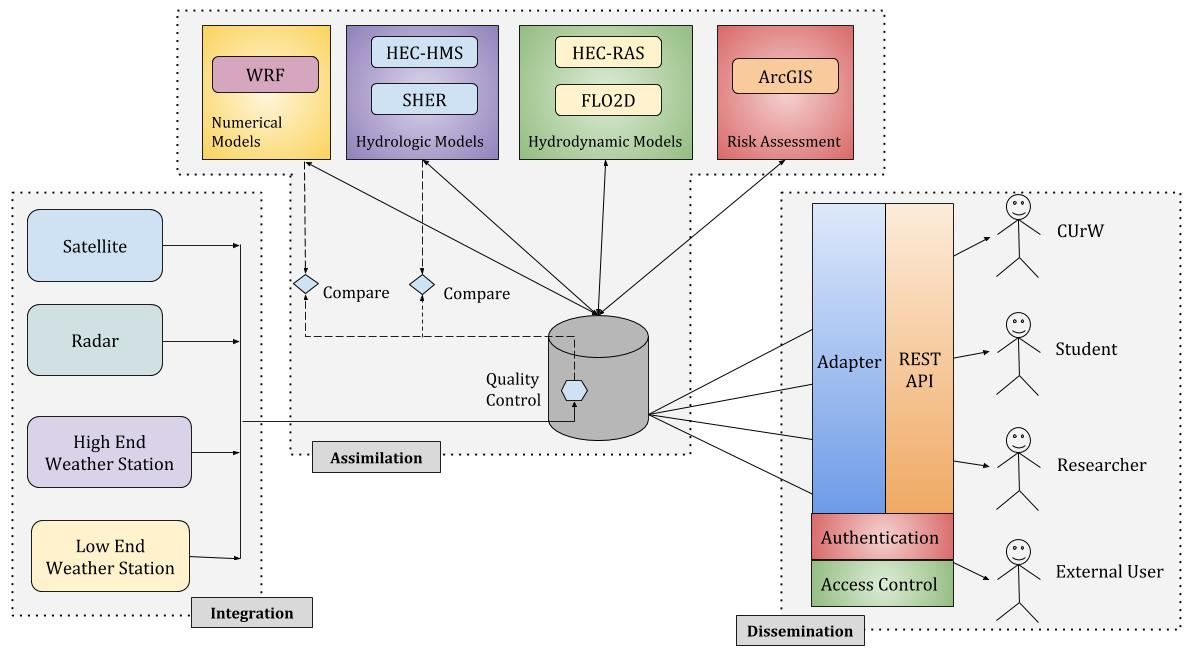
\includegraphics[width=0.5\textwidth]{method/misc/weather_data_system_components.jpg}}
\caption{Components of a Weather Data System.}
\label{fi:wdia_components}
\end{figure}
\paragraph{Integration} The system should capable of integrating data from different source such as satellite data, high end and low end weather station etc. And the system should be able to handle multidimensional spatial and temporal weather data efficiently and optimally. 
\paragraph{Assimilation} Then the system should be able to fulfill weather models varying data requirements. Also those models reproduce large set of redundant data, thus system should store the bulk data while optimizing the disk space.
\paragraph{Dissemination} Then different users should be able to retrieve data as they required. Also the users should be able to easy to search into the available that in the system base on timeseries metadata or based on Geo queries.

%%%%%%%%%%%%%%%%%%%%%%%%%%%%%%%%%%%%%%%%%%%%%%%%%%%%%%%%%%%%%%%%%%%%%%%%%%%%%%%%
\section{Different Architectures}

\subsection{\acrfull{soa}}
\begin{figure}[htbp]
\centerline{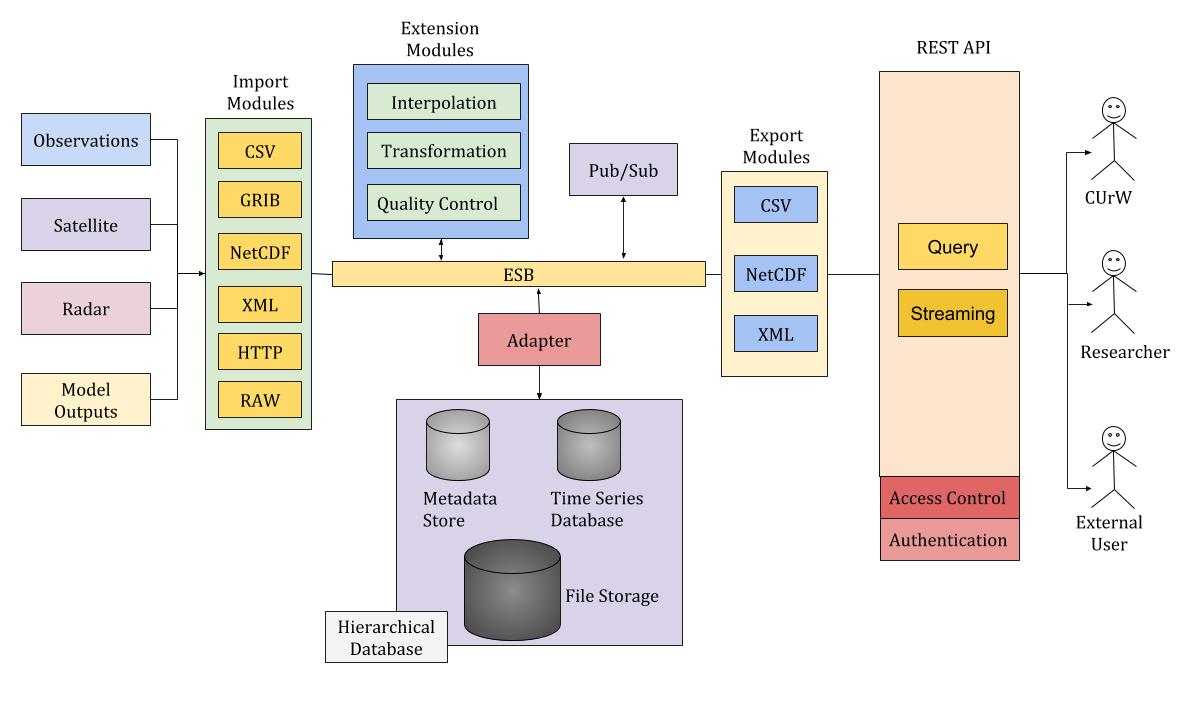
\includegraphics[width=0.5\textwidth]{method/soa/soa_v1.jpg}}
\caption{Proposed \acrshort{soa} Architecture for \acrshort{wdias}.}
\label{fi:wdias_soa_architecture}
\end{figure}

\subsection{Actor Model}


\subsection{Microservice Architecture}
\begin{figure}[htbp]
\centerline{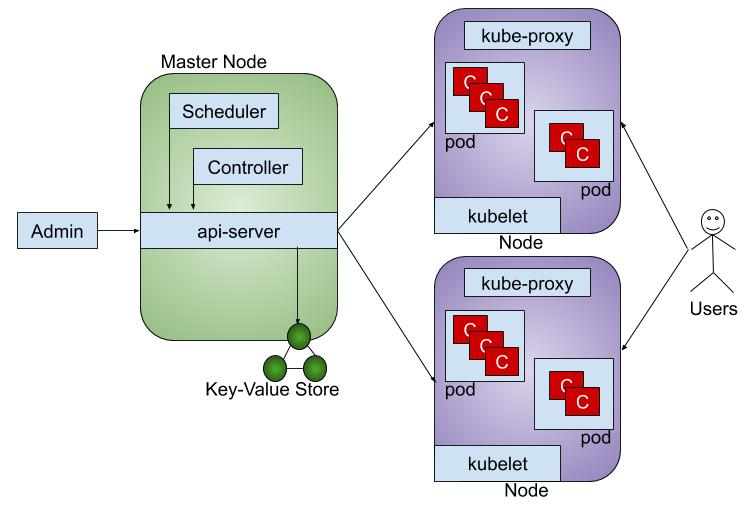
\includegraphics[width=0.5\textwidth]{method/microservice/k8s_architecture_v3.jpg}}
\caption{\acrfull{k8s} Architecture.}
\label{fi:k8s_architecture}
\end{figure}

%%%%%%%%%%%%%%%%%%%%%%%%%%%%%%%%%%%%%%%%%%%%%%%%%%%%%%%%%%%%%%%%%%%%%%%%%%%%%%%%
\section{Structure of \acrshort{wdias}}
\begin{figure}[htbp]
\centerline{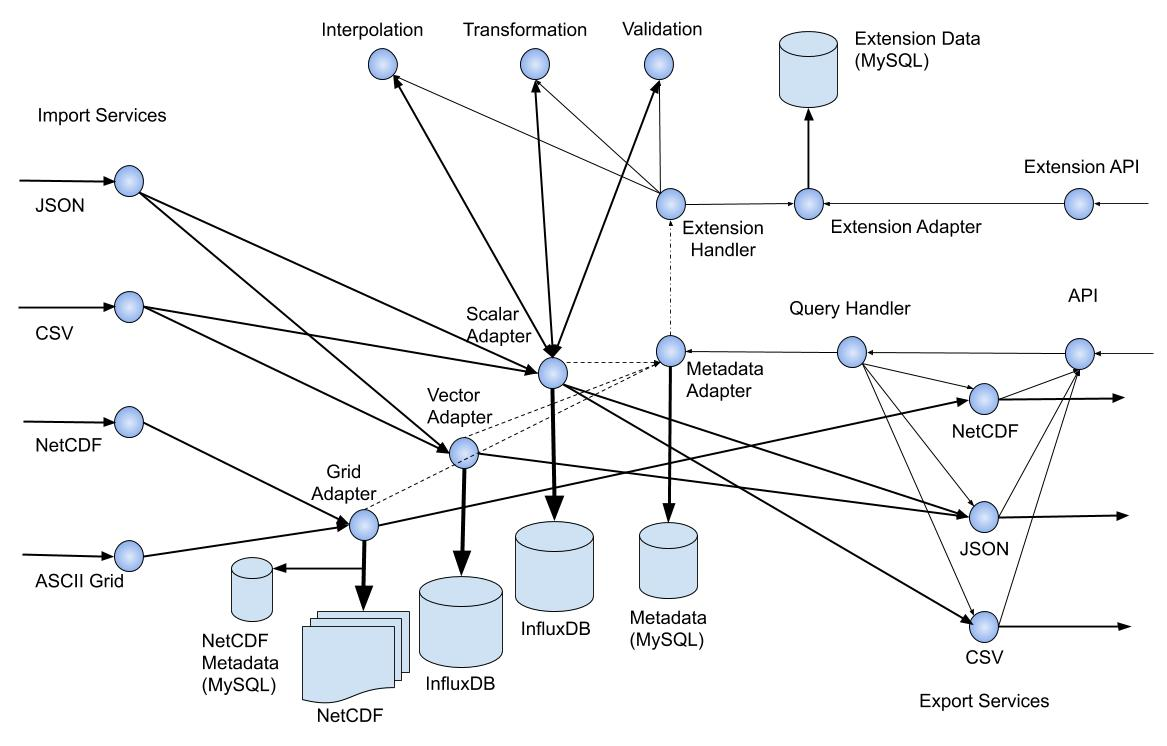
\includegraphics[width=0.5\textwidth]{method/microservice/microservice_architecture-handle_on_demand-v3.jpg}}
\caption{microservice Architecture - Handle on Demand.}
\label{fi:microservice_architecture_on_demand}
\end{figure}

\begin{figure}[htbp]
\centerline{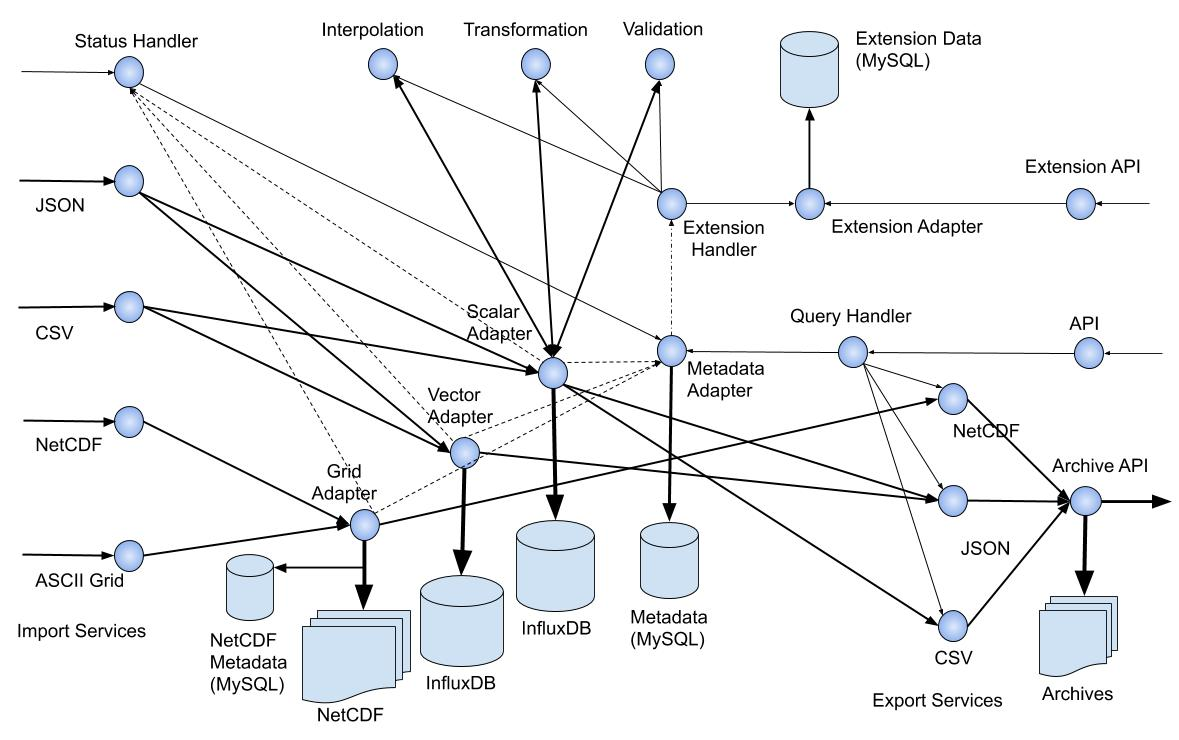
\includegraphics[width=0.5\textwidth]{method/microservice/microservice_architecture-handle_on_async-v3.jpg}}
\caption{microservice Architecture - Handle Asynchronously.}
\label{fi:microservice_architecture_async}
\end{figure}

\subsection{Hierarchical Database Structure}
\begin{figure}[htbp]
\centerline{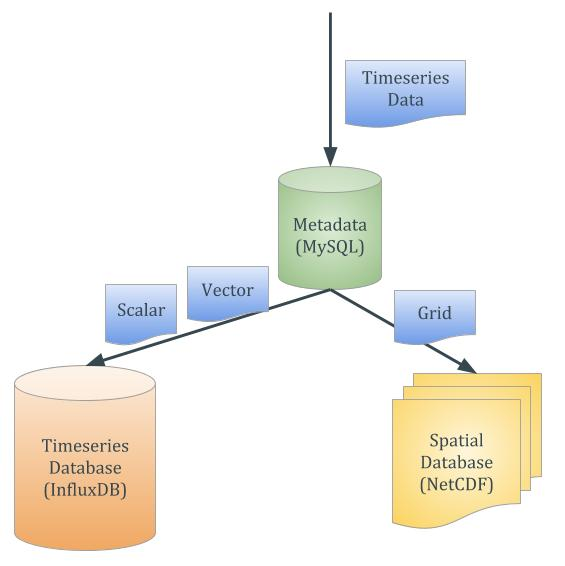
\includegraphics[width=0.4\textwidth]{method/microservice/hierarchical_database.jpg}}
\caption{Hierarchical Database.}
\label{fi:hierarchical_database}
\end{figure}

\subsection{Weather Data Preprocessing}
\begin{figure}[htbp]
\centerline{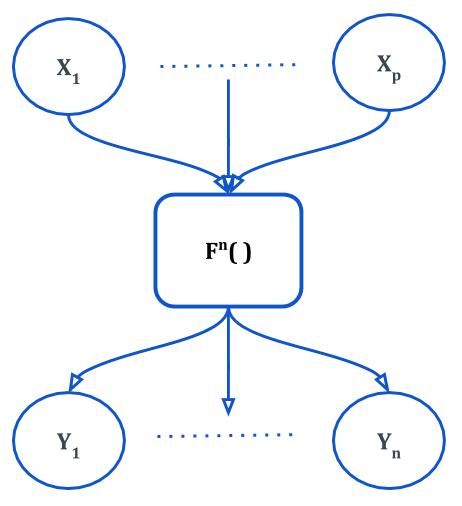
\includegraphics[width=0.5\textwidth]{method/data_preprocess/weather_data_preprocessing.jpg}}
\caption{Generic Functional Approach to Weather data preprocessing.}
\label{fi:weather_Data_preprocessing}
\end{figure}

\subsection{Query Timeseries Metadata}


%%%%%%%%%%%%%%%%%%%%%%%%%%%%%%%%%%%%%%%%%%%%%%%%%%%%%%%%%%%%%%%%%%%%%%%%%%%%%%%%
\section{Performance Analysis}

\subsection{Test Plan and Work Load}
\begin{figure}[htbp]
\centerline{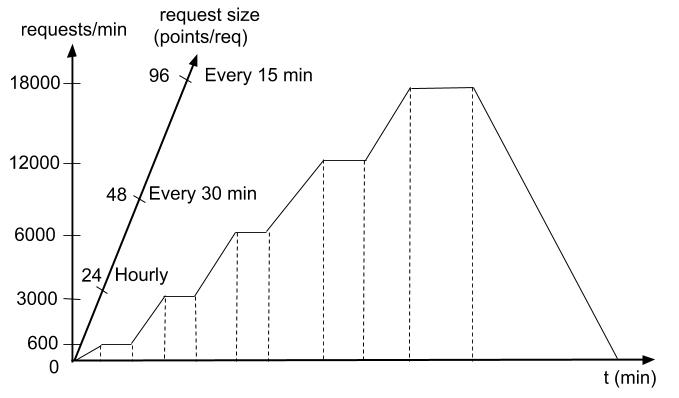
\includegraphics[width=0.5\textwidth]{results/work_load/performance_study_v4.jpg}}
\caption{Performance Study.}
\label{fi:performance_Study}
\end{figure}

\subsection{Observations}
\begin{table}[htbp]
\caption{Table Type Styles}
\begin{center}
\begin{tabular}{|c|c|c|c|c|c|c|}
\hline
\textbf{Label} & \textbf{Samples} & \textbf{Avg} & \textbf{Min} & \textbf{Max} & \textbf{Std} & \textbf{90\% Line} \\ \hline
Insert Scalar & 71727 & 34 & 13 & 1777 & 118.78 & 27 \\ \hline
Retrieve Scalar & 71693 & 7 & 5 & 1608 & 18.72 & 9 \\ \hline
Insert Grid & 7968 & 87 & 77 & 233 & 14.07 & 98 \\ \hline
Retrieve Grid & 7965 & 89 & 63 & 1694 & 37.79 & 110 \\ \hline
Query & 71704 & 1 & 0 & 203 & 2.05 & 2 \\ \hline
\textbf{TOTAL} & 310734 & 130 & 0 & 1777 & 212.35 & 501 \\ \hline
\multicolumn{4}{l}{$^{\mathrm{a}}$Avg: Average Latency, Std: Standard Deviation.}
\end{tabular}
\label{tab:obs_all_auto_15_min_summary_latency}
\end{center}
\end{table}

\begin{table}[htbp]
\caption{Table Type Styles}
\begin{center}
\begin{tabular}{|c|c|c|c|c|c|}
\hline
\textbf{Label} & \textbf{Samples} & \textbf{Avg} & \textbf{Std. Dev.} & \textbf{Error \%} & \textbf{RPS} \\ \hline
Insert Scalar & 71727 & 34 & 118.78 & 0.00\% & 40.5 \\ \hline
Retrieve Vector & 71693 & 7 & 18.72 & 0.00\% & 40.5 \\ \hline
Insert Grid & 7968 & 87 & 14.07 & 0.18\% & 4.5 \\ \hline
Retrieve Grid & 7965 & 89 & 37.79 & 0.00\% & 4.5 \\ \hline
Query & 71704 & 1 & 2.05 & 0.00\% & 40.5 \\ \hline
\textbf{TOTAL} & 310734 & 130 & 212.35 & 0.00\% & 175.3 \\ \hline
\multicolumn{4}{l}{$^{\mathrm{a}}$Avg: Average Latency.}
\end{tabular}
\label{tab:obs_all_auto_15_min_summary_throughput}
\end{center}
\end{table}

\begin{figure}[htbp]
\centerline{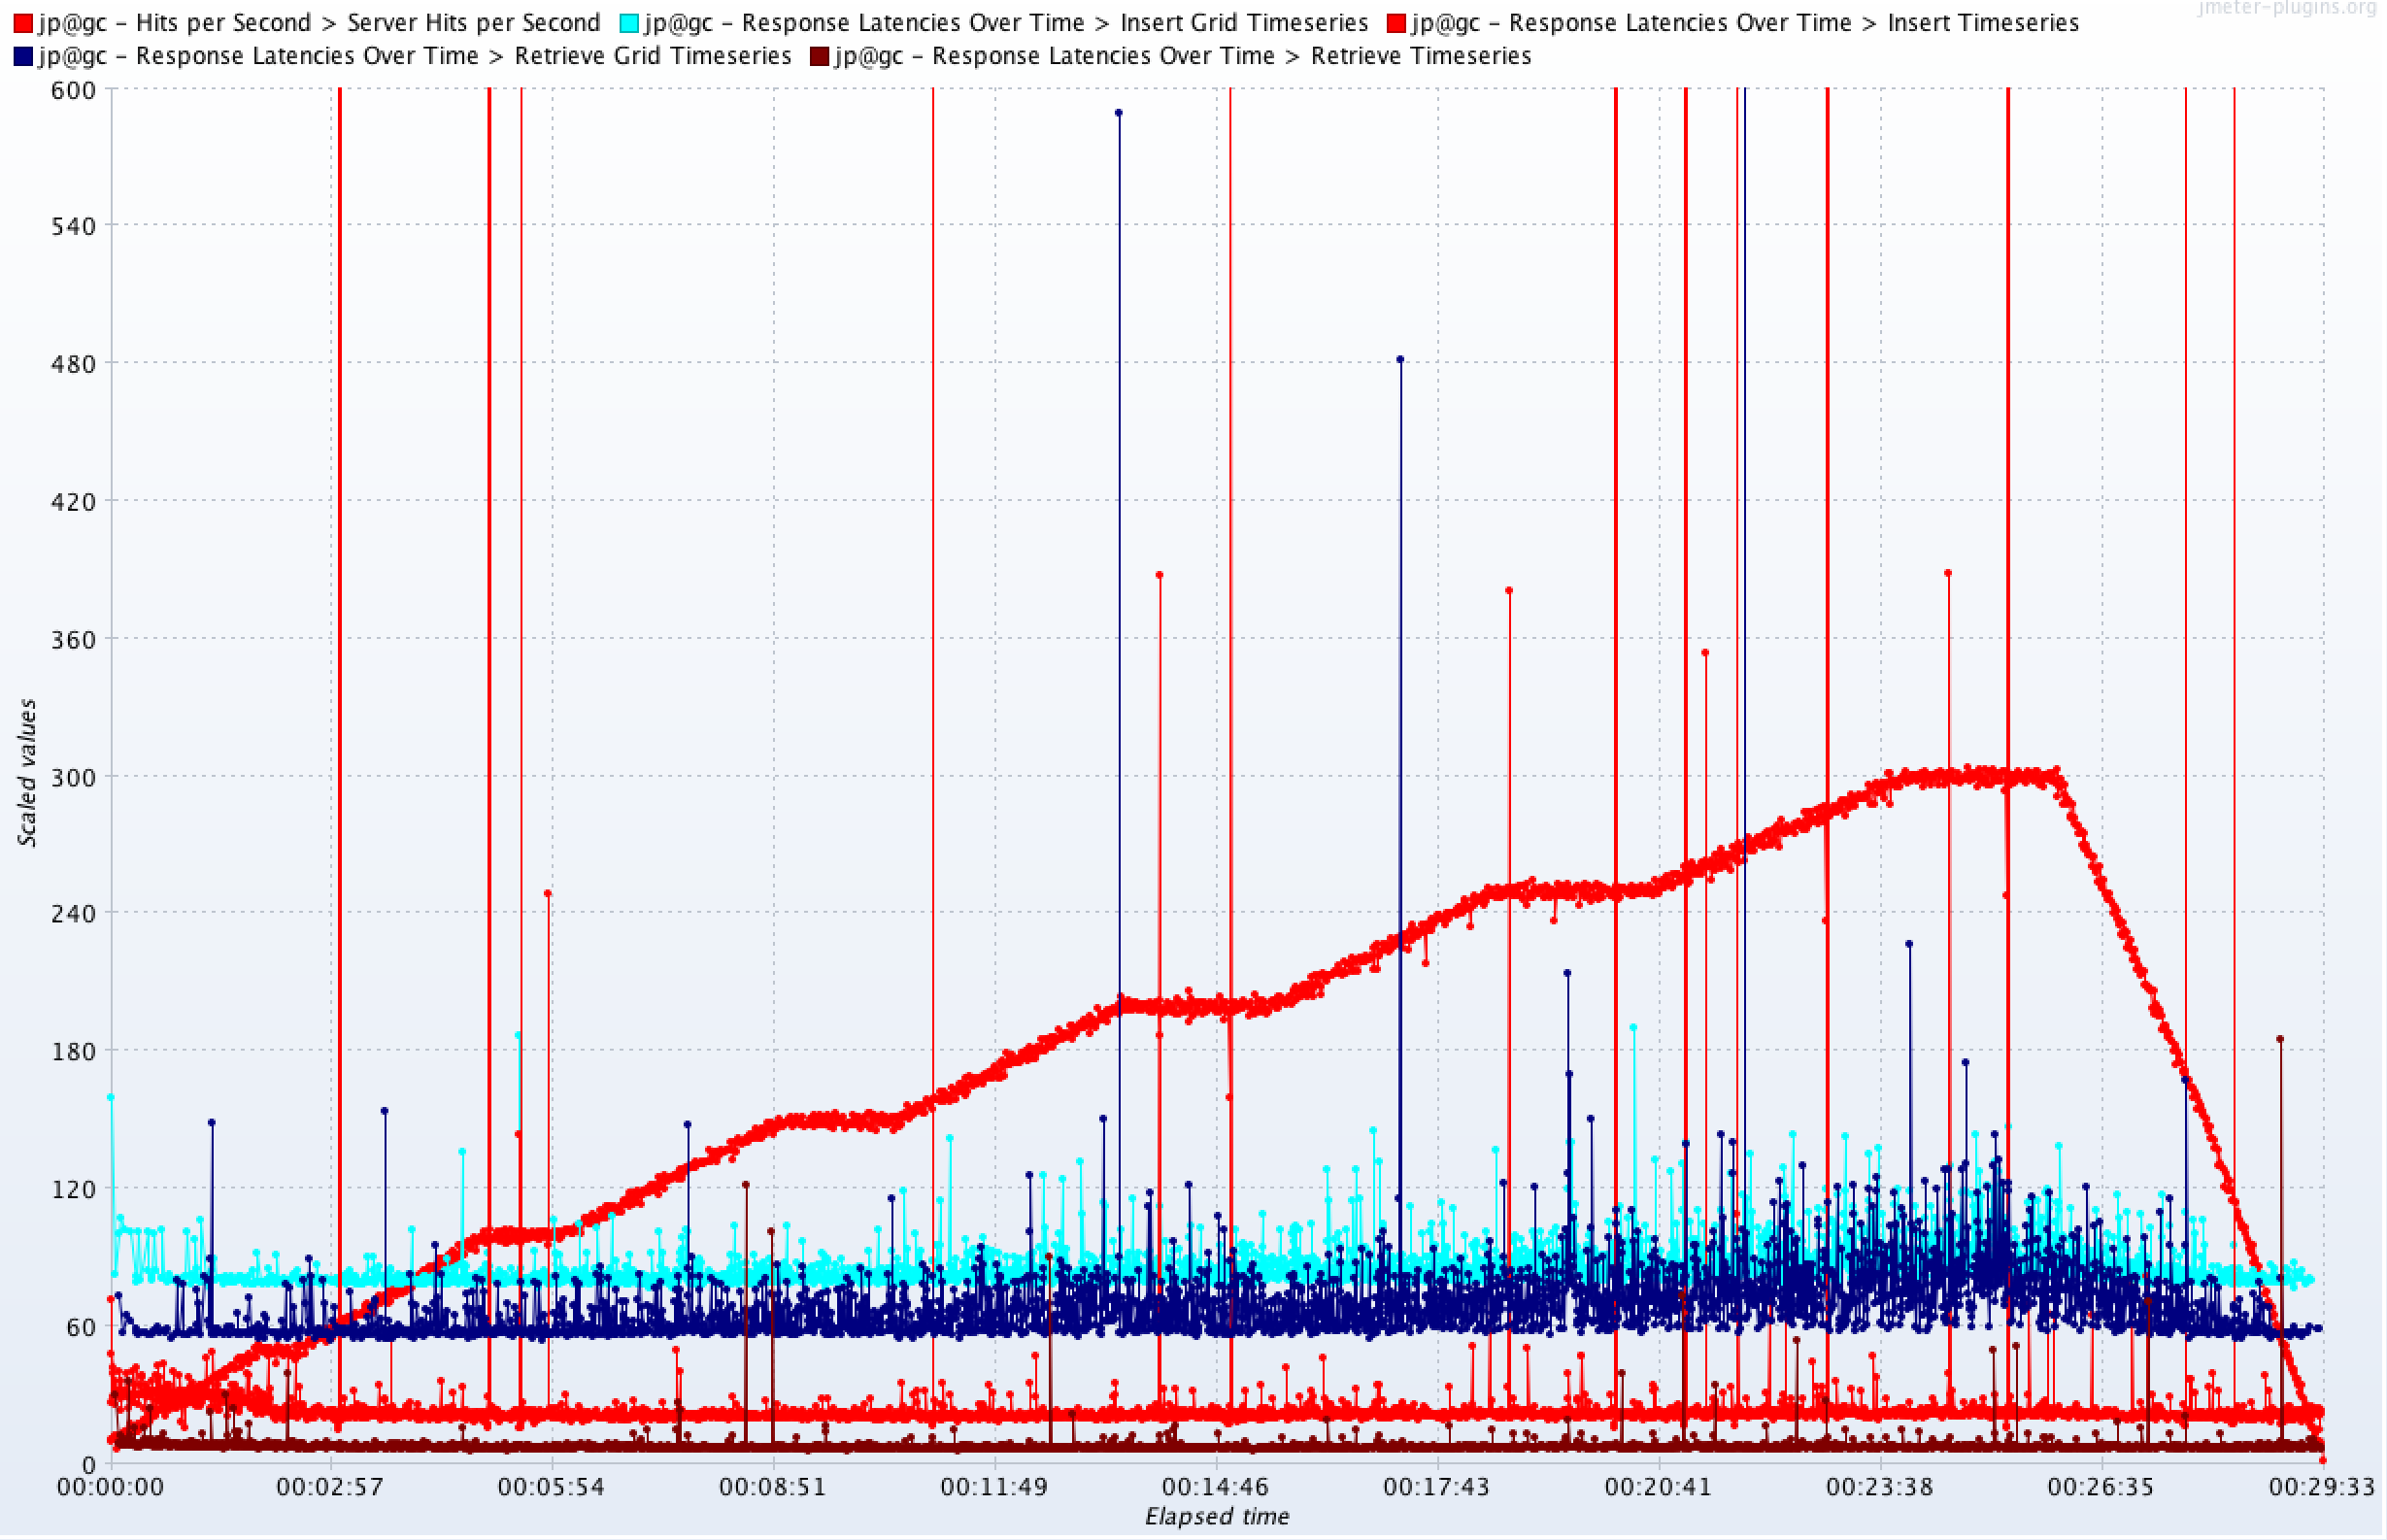
\includegraphics[width=0.5\textwidth]{results/obs/all_auto/obs_all_auto_15m_res_latencies_against_hits.png}}
\caption{Performance Test 15min data enabled Auto Scaling - Response Latencies against Server Hits over the elapsed time.}
\label{fi:test_obs_auto_all_15_min_latency_vs_hits}
\end{figure}

\begin{figure}[htbp]
\centerline{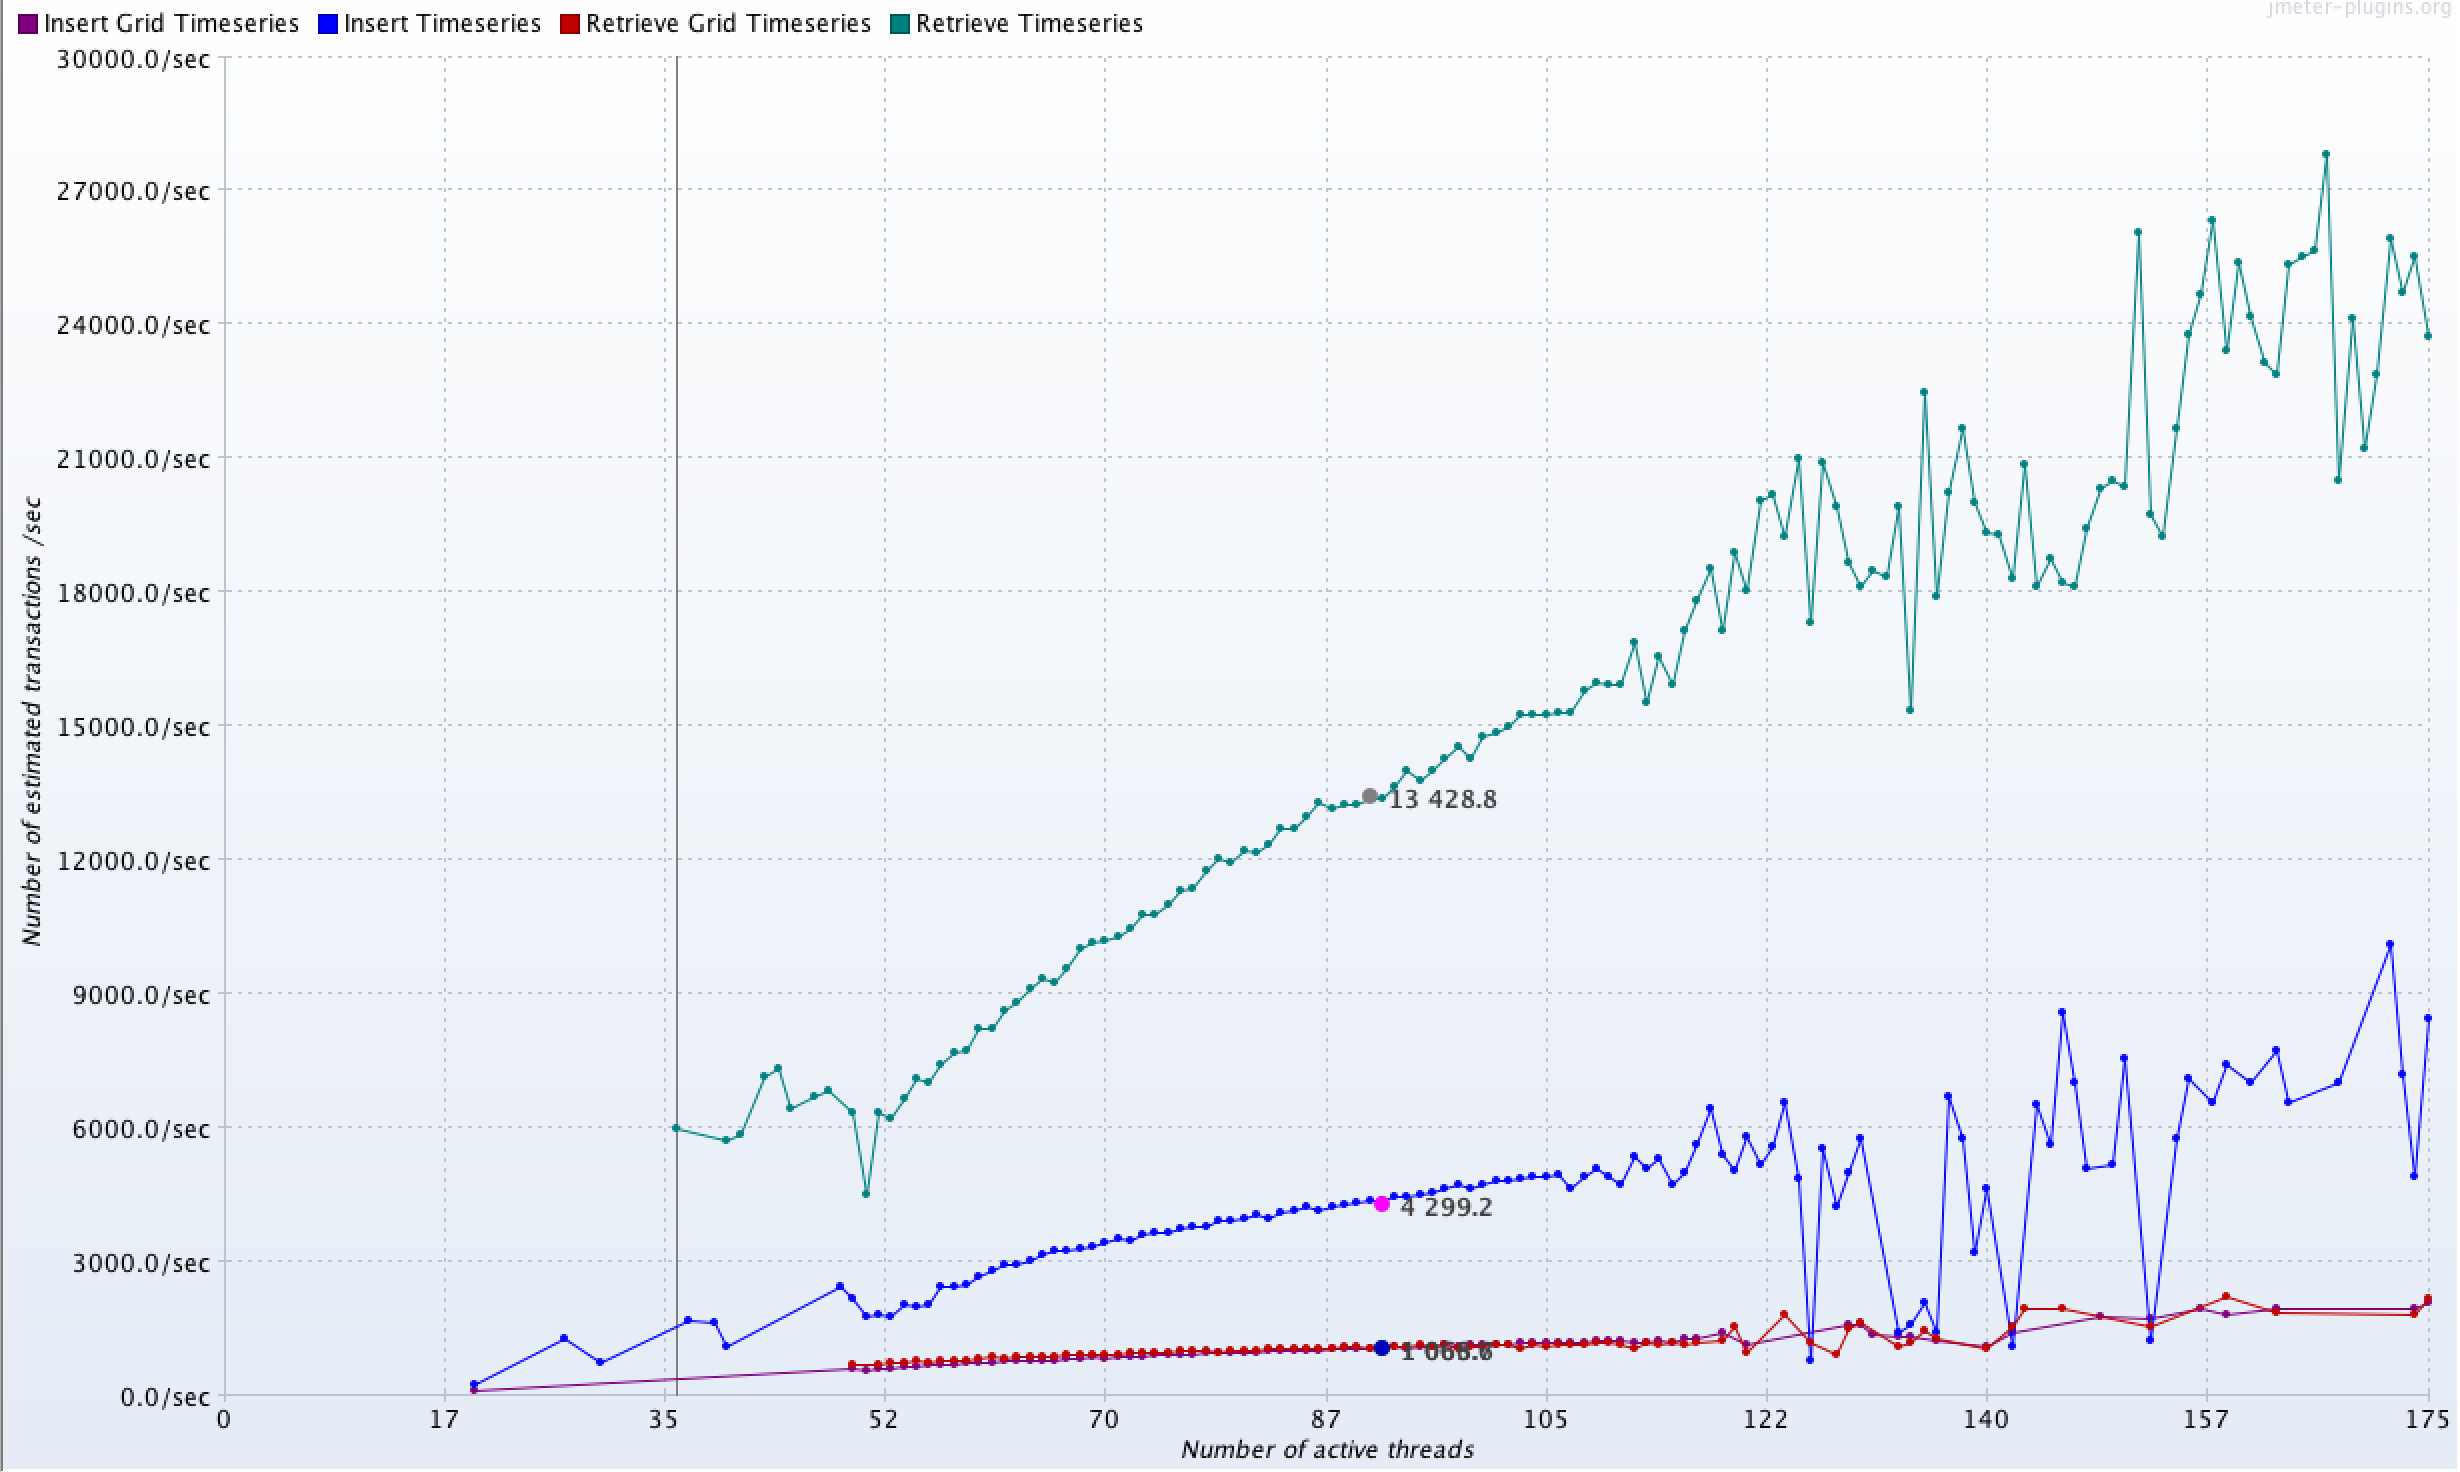
\includegraphics[width=0.5\textwidth]{results/obs/all_auto/obs_all_auto_15m_transaction_throughtput_vs_threads.png}}
\caption{Performance Test 15min data enabled Auto Scaling - Transnational Throughput vs Number of Active Threads.}
\label{fi:test_obs_auto_all_15_min_throughput_vs_threads}
\end{figure}

\subsection{Conclusion}


%%%%%%%%%%%%%%%%%%%%%%%%%%%%%%%%%%%%%%%%%%%%%%%%%%%%%%%%%%%%%%%%%%%%%%%%%%%%%%%%
\section{Strengths and Limitations}


%%%%%%%%%%%%%%%%%%%%%%%%%%%%%%%%%%%%%%%%%%%%%%%%%%%%%%%%%%%%%%%%%%%%%%%%%%%%%%%%
\section{Summary}


%%%%%%%%%%%%%%%%%%%%%%%%%%%%%%%%%%%%%%%%%%%%%%%%%%%%%%%%%%%%%%%%%%%%%%%%%%%%%%%%
\section*{Acknowledgment}

The preferred spelling of the word ``acknowledgment'' in America is without 
an ``e'' after the ``g''. Avoid the stilted expression ``one of us (R. B. 
G.) thanks $\ldots$''. Instead, try ``R. B. G. thanks$\ldots$''. Put sponsor 
acknowledgments in the unnumbered footnote on the first page.


%%%%%%%%%%%%%%%%%%%%%%%%%%%%%%%%%%%%%%%%%%%%%%%%%%%%%%%%%%%%%%%%%%%%%%%%%
\graphicspath{ {./images/} }
\bibliographystyle{plain}
\bibliography{mendeley}

\end{document}
